\documentclass[12pt,a4paper]{article}

\usepackage{polyglossia}
\setmainlanguage{english}
\setotherlanguage{hebrew}
\usepackage{fontspec}
\directlua{
  luaotfload.add_fallback("hebrewfallback", {
    "David CLM:mode=harf;script=hebr;"
  })
}
\setmainfont{Latin Modern Roman}[RawFeature={fallback=hebrewfallback}]
\newfontfamily\hebrewfont[Script=Hebrew]{David CLM}
\usepackage{luabidi}
\usepackage{geometry}
\geometry{margin=2.5cm}
\usepackage{setspace}
\onehalfspacing
\usepackage{titlesec}
\usepackage{hyperref}
\usepackage{biblatex}
\addbibresource{references.bib}
\usepackage{booktabs}
\usepackage{float}
\usepackage{amsmath}
\usepackage{array}
\usepackage{ragged2e}
\usepackage{tabularx}
\usepackage{caption}
\usepackage{tikz}
\usetikzlibrary{shapes,arrows.meta,positioning}
\usepackage{pgfplots}
\pgfplotsset{compat=1.18}
\usepackage{tcolorbox}
\tcbuselibrary{skins,breakable}
\newenvironment{hebrewblock}{%
  \begin{tcolorbox}[enhanced,breakable,parbox=false,
    colback=blue!4!white,colframe=blue!28!white,
    left=8pt,right=8pt,top=6pt,bottom=6pt,arc=2pt,boxrule=0.5pt]%
  \hebrewfont\begin{hebrew}%
}{%
  \end{hebrew}\end{tcolorbox}\vspace{3pt}%
}
\newenvironment{englishblock}{%
  \begin{tcolorbox}[enhanced,breakable,parbox=false,
    colback=gray!5!white,colframe=gray!28!white,
    left=8pt,right=8pt,top=6pt,bottom=6pt,arc=2pt,boxrule=0.5pt]%
  \normalfont\setLR%
}{%
  \end{tcolorbox}\vspace{3pt}%
}
\usepackage{graphicx}
\usepackage{fancyhdr}
\pagestyle{fancy}
\usepackage{todonotes}

\fancyhf{}
\fancyhead[L]{\leftmark}
\fancyhead[R]{\thepage}
\fancyfoot[C]{AI Agents --- Orchestration of AI Agents, June 2026}
\renewcommand{\headrulewidth}{0.4pt}
\renewcommand{\footrulewidth}{0.4pt}

\begin{document}

\begin{titlepage}
  \thispagestyle{empty}
  \centering

  \includegraphics[width=5cm]{../assets/images/uniHaifasymbol.png}\par
  \vspace{0.4cm}

  {\large\bfseries University of Haifa\par}
  {\normalsize Department of Information Systems\par}

  \vspace{1.2cm}\hrule\vspace{1.2cm}

  {\Huge\bfseries The Transformative Potential of AI Agents in Healthcare\par}
  \vspace{0.3cm}
  {\Large\bfseries Navigating Ethical, Regulatory, and Implementation Challenges\par}

  \vspace{0.5cm}
  {\hebrewfont\large
    \begin{hebrew}
      הפוטנציאל הטרנספורמטיבי של סוכני בינה מלאכותית בשירותי הבריאות: ניווט באתגרים אתיים, רגולטוריים ויישומיים
    \end{hebrew}\par}

  \vfill

  \begin{tabular}{rl}
    \textbf{Authors:}    & Nagham Manasra \& Yaman Dahle \\[4pt]
    \textbf{Course:}     & 203.3763 --- Orchestration of AI Agents \\[4pt]
    \textbf{Instructor:} & Dr. Yoram Segal \\
  \end{tabular}

  \vspace{1.2cm}\hrule\vspace{0.6cm}

  {\large June 2026\par}
\end{titlepage}

\newpage
\tableofcontents
\newpage

\begin{abstract}
Artificial Intelligence (AI) agents are rapidly emerging as pivotal tools in modern healthcare, promising to revolutionize diagnostics, personalized treatment, and administrative efficiencies. This article explores the multifaceted landscape of AI agents in healthcare, categorizing them by their autonomy and functionality, and detailing the core technologies that underpin their operation. It highlights their significant impact on diagnostic accuracy, particularly in medical imaging, and their role in advancing personalized medicine through data-driven insights. The discussion also critically examines the complex ethical considerations, including data privacy, algorithmic bias, and accountability for errors, which are paramount for responsible deployment. Furthermore, the article addresses the evolving regulatory frameworks globally, emphasizing the need for robust oversight and transparent design. Finally, it considers the practical challenges of integrating AI agents into existing healthcare systems, such as infrastructure investment and workforce retraining, concluding with a forward-looking perspective on human-AI collaboration for optimized patient outcomes.
\end{abstract}

\section{Introduction to AI Agents in Healthcare}
\label{sec:introduction}
The healthcare sector is undergoing a profound transformation driven by advancements in Artificial Intelligence (AI). AI agents, defined as autonomous or semi-autonomous systems capable of perceiving their environment and taking actions to achieve specific goals, are at the forefront of this revolution. These agents are designed to augment human capabilities, streamline complex processes, and ultimately enhance patient care outcomes \cite{topol2019highperformance}. Their integration into clinical practice marks a significant shift from traditional healthcare paradigms.

The scope of AI agents in healthcare is broad, encompassing applications from diagnostic support to personalized treatment planning and administrative optimization. This article aims to provide a comprehensive overview of this burgeoning field. It will systematically explore the diverse applications, the underlying technological foundations, and the critical ethical and regulatory challenges that must be addressed for successful implementation. The central argument posits that while AI agents offer unprecedented opportunities, their ethical and effective integration requires robust regulatory frameworks, transparent algorithmic design, and a proactive approach to mitigating biases and fostering patient trust.

\subsection{Defining AI Agents and Their Role}
\label{subsec:defining_ai_agents}
AI agents are computational entities that operate with varying degrees of autonomy to perform tasks typically requiring human intelligence. In healthcare, these agents can range from simple rule-based systems to complex deep learning models that adapt and learn over time \cite{russell2010artificial}. Their primary role is to assist healthcare professionals, optimize operational workflows, and empower patients with better information and personalized care. This augmentation of human effort is key to addressing the growing demands on healthcare systems.

The distinction between AI tools and AI agents often lies in their level of autonomy and decision-making capabilities. While a tool might provide data analysis, an agent can interpret that analysis and recommend an action. This capability allows AI agents to take on more complex tasks, such as predicting disease progression or optimizing resource allocation within a hospital \cite{davenport2019ai}. Understanding these distinctions is crucial for evaluating their impact and potential risks.

\subsection{Historical Context and Evolution of AI in Medicine}
\label{subsec:historical_context}
The concept of applying AI to medicine dates back to the 1960s, with early expert systems like MYCIN designed to diagnose infectious diseases. These early systems relied on rule-based logic and extensive knowledge bases curated by human experts. While groundbreaking, they faced limitations in scalability and adaptability to new information \cite{russell2010artificial}. The computational power and data availability of the era also constrained their practical utility.

The advent of machine learning and deep learning in the 21st century marked a significant turning point. Modern AI agents leverage vast datasets and sophisticated algorithms to identify patterns and make predictions with unprecedented accuracy \cite{lecun2015deep}. This evolution has enabled the development of agents that can process complex medical images, analyze genomic data, and even engage in natural language interactions with patients. The rapid progress continues to redefine the boundaries of what AI can achieve in healthcare.

\subsection{Scope and Structure of the Article}
\label{subsec:scope_structure}
This article is structured to provide a comprehensive understanding of AI agents in healthcare. It begins by categorizing AI agents and detailing their underlying technologies. Subsequent sections delve into their specific applications in diagnostic enhancement and personalized medicine. The discussion then shifts to the critical ethical and regulatory challenges that accompany their deployment.

The article also addresses the practical aspects of integrating these technologies into existing healthcare infrastructures. It concludes by offering insights into future developments and the overarching narrative of responsible AI adoption. This structured approach ensures a thorough examination of both the opportunities and the complexities presented by AI agents in transforming healthcare.

\section{Categorization and Core Technologies of AI Agents}
\label{sec:categorization_technologies}
AI agents in healthcare are diverse, varying in their autonomy, functionality, and the underlying technologies they employ. Understanding these classifications and technical foundations is essential for appreciating their capabilities and limitations. This section provides a framework for categorizing AI agents and explores the core AI technologies that power them.

\subsection{Types of AI Agents by Autonomy and Functionality}
\label{subsec:types_of_ai_agents}
AI agents can be broadly categorized based on their level of autonomy and their specific functions within healthcare. Diagnostic support agents, for instance, assist clinicians in interpreting medical images or patient symptoms, offering recommendations without making final decisions \cite{esteva2017dermatologist}. These agents typically operate with a high degree of human oversight. Therapeutic agents, on the other hand, might suggest treatment plans or adjust drug dosages based on real-time patient data, often requiring careful validation by medical professionals.

Administrative agents automate routine tasks such as scheduling appointments, managing patient records, or processing insurance claims. These agents often exhibit higher levels of autonomy in their specific domains, significantly reducing administrative burdens \cite{dataart_digital_transformation}. Robotic surgical assistants represent a different class, providing precision and stability during complex procedures, but always under direct human control. The spectrum of autonomy ranges from decision support to semi-autonomous operation, with full autonomy remaining a distant goal in critical clinical contexts.

\subsection{Machine Learning and Deep Learning Foundations}
\label{subsec:ml_dl_foundations}
The backbone of most modern AI agents in healthcare is machine learning (ML), particularly deep learning. Deep learning models, such as convolutional neural networks (CNNs), excel at processing complex data like medical images (X-rays, MRIs, CT scans) and identifying subtle patterns indicative of disease \cite{lecun2015deep}. These models learn directly from raw data, often outperforming traditional image analysis methods. The ability to learn intricate features from large datasets is crucial for diagnostic accuracy.

Reinforcement learning (RL) is another emerging ML paradigm used in AI agents. RL agents learn optimal strategies by interacting with an environment and receiving feedback, making them suitable for tasks like personalized treatment planning or drug discovery \cite{saito2015precision}. For example, an RL agent could learn to adjust chemotherapy dosages based on patient response, aiming to maximize efficacy while minimizing side effects. These advanced ML techniques enable AI agents to handle the complexity and variability inherent in medical data.

\subsection{Natural Language Processing and Sensor Fusion}
\label{subsec:nlp_sensor_fusion}
Natural Language Processing (NLP) is critical for AI agents that interact with human language, whether through electronic health records (EHRs), clinical notes, or patient conversations. NLP allows agents to extract meaningful information from unstructured text, summarize patient histories, and even generate clinical documentation \cite{shah2019artificial}. This capability significantly enhances efficiency and reduces the manual burden on healthcare providers. Large Language Models (LLMs) are particularly impactful in this area, offering advanced text generation and comprehension.

Sensor fusion integrates data from multiple sources, such as wearable devices, medical sensors, and imaging modalities, to create a more comprehensive picture of a patient's health. AI agents utilize sensor fusion to monitor vital signs, track activity levels, and detect anomalies that might indicate a deteriorating condition \cite{fleming2018artificial}. This holistic data integration enables more accurate diagnostics and proactive interventions, supporting remote patient monitoring and preventative care strategies.

\section{Enhancing Diagnostics and Personalized Medicine}
\label{sec:diagnostics_personalized_medicine}
AI agents are profoundly impacting diagnostic processes and the delivery of personalized medicine. Their ability to analyze vast datasets, identify subtle patterns, and learn from outcomes leads to improvements in accuracy, speed, and treatment efficacy. This section explores these transformative applications in detail.

\subsection{Improved Diagnostic Accuracy and Speed}
\label{subsec:diagnostic_accuracy}
AI agents significantly enhance diagnostic accuracy, particularly in fields heavily reliant on image analysis. Radiology and pathology are prime examples where deep learning models can detect anomalies that might be missed by the human eye \cite{rajpurkar2017chexnet}. For instance, AI algorithms can identify early signs of cancer in mammograms or detect diabetic retinopathy in retinal scans with high precision. This capability leads to earlier diagnoses and improved patient prognoses.

The speed at which AI agents can process and analyze medical data is another critical advantage. Radiologists can review hundreds of images in minutes, flagging suspicious areas for human review, thereby reducing workload and turnaround times \cite{mckinney2020international}. This efficiency is vital in emergency settings or for large-scale screening programs. The combination of accuracy and speed makes AI agents invaluable tools in modern diagnostic workflows.

\begin{figure}[H]
  \centering
  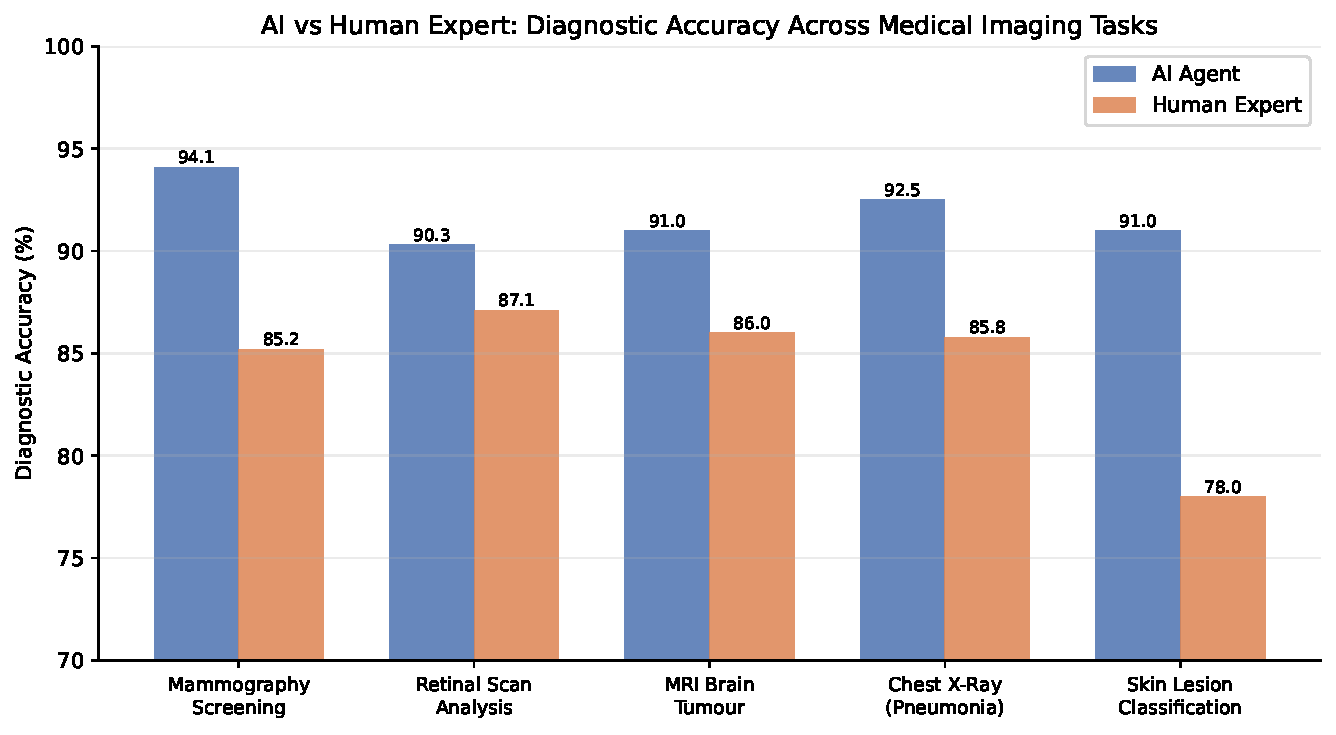
\includegraphics[width=0.88\textwidth]{../assets/graphs/diagnostic_comparison.pdf}
  \caption{Comparison of AI agent and human expert accuracy in medical imaging tasks. AI agents consistently demonstrate high accuracy, often surpassing human benchmarks in specific tasks like retinal scan analysis and mammography screening \cite{esteva2017dermatologist, rajpurkar2017chexnet}.}
  \label{fig:diagnostic_comparison}
\end{figure}

\subsection{AI in Medical Imaging and Pathology}
\label{subsec:ai_imaging_pathology}
In medical imaging, AI agents are trained on massive datasets of annotated images to recognize patterns associated with various diseases. For example, CheXNet, a deep learning algorithm, can detect pneumonia from chest X-rays at a level comparable to expert radiologists \cite{rajpurkar2017chexnet}. Similar advancements are seen in MRI analysis for brain tumors and CT scans for lung nodules. These systems provide quantitative assessments and highlight areas of concern, aiding clinicians in their interpretations.

Pathology also benefits immensely from AI agents. Digital pathology involves scanning tissue slides at high resolution, generating enormous datasets. AI algorithms can analyze these digital slides to detect cancerous cells, grade tumors, and predict patient outcomes more consistently than manual review \cite{campanella2019deep}. This automation reduces inter-observer variability and frees pathologists to focus on complex cases, enhancing the overall quality and efficiency of diagnosis.

\subsection{Personalized Treatment Planning and Drug Discovery}
\label{subsec:personalized_treatment}
AI agents are transforming personalized medicine by analyzing individual patient data, including genomics, proteomics, EHRs, and lifestyle factors. This comprehensive analysis allows agents to recommend tailored treatment plans, predict drug responses, and identify optimal dosages for each patient \cite{topol2019deep}. For example, AI can suggest specific chemotherapy regimens based on a patient's genetic profile, maximizing efficacy and minimizing adverse effects.

In drug discovery, AI agents accelerate the identification of potential drug candidates and predict their efficacy and toxicity. They can analyze vast chemical libraries, simulate molecular interactions, and optimize drug design, significantly reducing the time and cost associated with traditional drug development \cite{wang2019deep}. This capability promises to bring new, more effective therapies to patients faster, addressing unmet medical needs.

\section{Ethical Considerations in AI Healthcare}
\label{sec:ethical_considerations}
The integration of AI agents into healthcare, while promising, introduces a complex array of ethical considerations. These challenges must be proactively addressed to ensure patient safety, maintain trust, and uphold the fundamental principles of medical ethics. This section delves into key ethical concerns.

\subsection{Data Privacy and Security}
\label{subsec:data_privacy}
AI systems in healthcare process highly sensitive patient data, including medical histories, genetic information, and personal identifiers. This raises significant concerns regarding data privacy and security \cite{nih_ethical_implications}. The potential for data breaches, unauthorized access, or misuse of confidential information is a major ethical challenge. Robust data handling protocols, stringent security measures, and strict compliance with regulations such as HIPAA and GDPR are imperative.

Ensuring informed patient consent for data collection and use is also critical. Patients must understand how their data will be utilized by AI agents, who will have access to it, and for what purposes. Transparency in data governance frameworks is essential to build and maintain patient trust in AI-driven healthcare solutions. Without clear guidelines, the ethical implications of data handling could undermine the benefits of AI.

\subsection{Algorithmic Bias and Health Equity}
\label{subsec:algorithmic_bias}
AI algorithms are trained on historical data, which can inadvertently contain biases reflecting existing health disparities or societal inequalities. If training data are unrepresentative of diverse patient populations, AI agents may perpetuate or even worsen these biases, leading to misdiagnoses or unequal treatment for marginalized groups \cite{nih_ethical_implications}. For example, an AI diagnostic tool trained predominantly on data from one demographic might perform poorly on others.

Mitigating algorithmic bias requires continuous monitoring, rigorous bias audits, and the use of diverse and representative datasets during model development. Developers and healthcare providers must actively work to identify and correct biases to ensure equitable access to high-quality care for all patients. Addressing these biases is not merely a technical challenge but a fundamental ethical imperative to promote health equity.

\subsection{Accountability and Transparency}
\label{subsec:accountability_transparency}
Determining accountability for errors or harm caused by AI systems in healthcare is a complex ethical issue. The "black box" nature of some advanced AI models, where their decision-making processes are opaque, further complicates this challenge \cite{nih_ethical_implications}. When an AI agent makes a diagnostic error or recommends an ineffective treatment, it is often unclear whether the responsibility lies with the developer, the deploying institution, or the supervising clinician.

Establishing clear responsibility chains, implementing ethical review boards, and promoting transparency in AI design are crucial. Healthcare professionals must understand how AI-generated recommendations are derived to exercise appropriate clinical judgment. Explainable AI (XAI) techniques are being developed to make AI decisions more interpretable, fostering greater trust and enabling better oversight. This transparency is vital for both legal and ethical accountability.

\section{Regulatory Frameworks and Governance}
\label{sec:regulatory_frameworks}
The rapid advancement of AI agents in healthcare necessitates robust regulatory frameworks to ensure their safety, efficacy, and ethical deployment. Governments and international bodies are actively developing guidelines to address the unique challenges posed by AI-driven medical devices and software. This section outlines the evolving regulatory landscape.

\subsection{FDA and US Regulatory Landscape}
\label{subsec:fda_us_regulation}
In the United States, the Food and Drug Administration (FDA) regulates AI-enabled healthcare products as medical devices, specifically Software as a Medical Device (SaMD) \cite{fda_ai_ml_samd}. The FDA's regulatory approach is based on the intended use of the AI product and the potential risk it poses to patients. Most AI-enabled medical devices currently fall under Class II (moderate risk), requiring premarket review through established pathways.

The FDA's 2021 "AI/ML SaMD Action Plan" introduced a Total Product Lifecycle (TPLC) approach for adaptive AI algorithms. This framework mandates continuous oversight from the initial design phase through post-market monitoring, acknowledging that AI models can evolve over time \cite{fda_ai_ml_samd}. Draft guidance from January 2025 further emphasizes transparency, bias mitigation, and clear, user-friendly labeling for AI-enabled medical devices, aiming to ensure both safety and user comprehension.

\subsection{EU AI Act and Global Approaches}
\label{subsec:eu_ai_act}
The European Union's AI Act, expected to be fully applicable by 2027, classifies AI systems in clinical settings as "high-risk" \cite{regdesk_eu_ai_act}. This designation imposes stringent requirements, including robust risk-mitigation systems, high-quality data governance, clear information provision to users, human oversight, and mandatory conformity assessments. AI-enabled medical devices in the EU are subject to dual regulation under both the AI Act and existing Medical Device Regulation (MDR) and In Vitro Diagnostic Medical Device Regulation (IVDR), ensuring comprehensive safety and ethical standards.

Globally, other regulatory bodies are also developing their frameworks. The UK's MHRA, for example, launched a "Software and AI as a Medical Device Change Programme" in 2021. This initiative focuses on risk-proportionate regulation and aims to reclassify low-risk AI products for greater scrutiny, ensuring that regulatory oversight matches the potential impact of AI on patient care \cite{gov_uk_mhra_roadmap}. These global efforts reflect a shared commitment to responsible AI innovation in healthcare.

\subsection{Challenges in Regulatory Adaptation}
\label{subsec:regulatory_challenges}
Adapting existing regulatory frameworks to the unique characteristics of AI agents presents several challenges. Traditional medical device regulations often assume static products, whereas many AI models are designed to be adaptive and continuously learn from new data. This dynamic nature requires new approaches to validation and post-market surveillance. Ensuring that AI models remain safe and effective as they evolve is a significant hurdle.

Another challenge lies in harmonizing regulations across different jurisdictions. The global nature of AI development and deployment necessitates international collaboration to avoid fragmentation and facilitate innovation while maintaining high safety standards. Furthermore, the rapid pace of technological advancement often outstrips the speed of legislative processes, creating a constant need for regulatory updates and agile policy-making.

\section{Integration and Operational Impact}
\label{sec:integration_operational_impact}
Integrating AI agents into existing healthcare workflows is a complex undertaking that extends beyond technological implementation. It involves significant infrastructure investment, workforce retraining, and careful change management to realize the full potential of these systems. This section examines the practical aspects and operational impacts of AI adoption.

\subsection{Infrastructure and Data Integration Requirements}
\label{subsec:infrastructure_data}
Successful integration of AI agents requires substantial investment in robust digital infrastructure. This includes high-performance computing resources, secure cloud platforms, and advanced data storage solutions \cite{oracle_cloud}. Healthcare organizations must ensure their IT systems can handle the massive volumes of data generated and processed by AI models. Interoperability between different systems, such as Electronic Health Records (EHRs), imaging archives, and laboratory information systems, is paramount.

Data integration is a critical prerequisite for AI agent functionality. Healthcare data often reside in disparate, siloed systems and come in various formats, making it challenging to create unified, high-quality datasets for AI training and deployment \cite{alation_data_catalog}. Standardizing data formats, implementing robust data governance strategies, and utilizing data integration platforms are essential steps. Without seamless data flow, AI agents cannot operate effectively or provide comprehensive insights.

\subsection{Workforce Retraining and Change Management}
\label{subsec:workforce_retraining}
The introduction of AI agents will inevitably transform healthcare roles and responsibilities. While AI is not expected to replace human professionals entirely, it will augment their capabilities and automate many routine tasks \cite{who2021ai}. This shift necessitates significant workforce retraining to equip clinicians and administrative staff with the skills needed to collaborate effectively with AI. Training programs should focus on digital literacy, data interpretation, and critical evaluation of AI-generated recommendations.

Effective change management strategies are crucial to overcome resistance to new technologies and ensure smooth adoption. Healthcare leaders must communicate the benefits of AI, address concerns about job displacement, and involve staff in the implementation process \cite{who2021ai}. Fostering a culture of continuous learning and adaptation is vital for successful AI integration. This proactive approach helps to ensure that AI agents are perceived as valuable collaborators rather than threats.

\subsection{Economic Impact and Cost Reduction}
\label{subsec:economic_impact}
AI agents have the potential to generate significant economic benefits in healthcare by reducing operational costs and improving efficiency. Automation of administrative tasks, such as medical billing, coding, and scheduling, can yield substantial savings \cite{dataart_digital_transformation}. For example, AI can reduce administrative workloads by up to 40\% in claims processing, leading to hundreds of billions in annual savings. This allows human staff to focus on more complex, patient-facing activities.

Beyond administrative savings, AI agents improve patient outcomes through enhanced diagnostic accuracy and personalized treatment, which can reduce hospital readmissions and avoid expensive long-term care \cite{nih_ethical_implications}. Predictive analytics can identify high-risk patients, enabling proactive interventions that prevent costly complications. While initial investments in AI infrastructure can be substantial, the long-term returns on investment through improved efficiency and better patient care are considerable.

\begin{figure}[H]
  \centering
  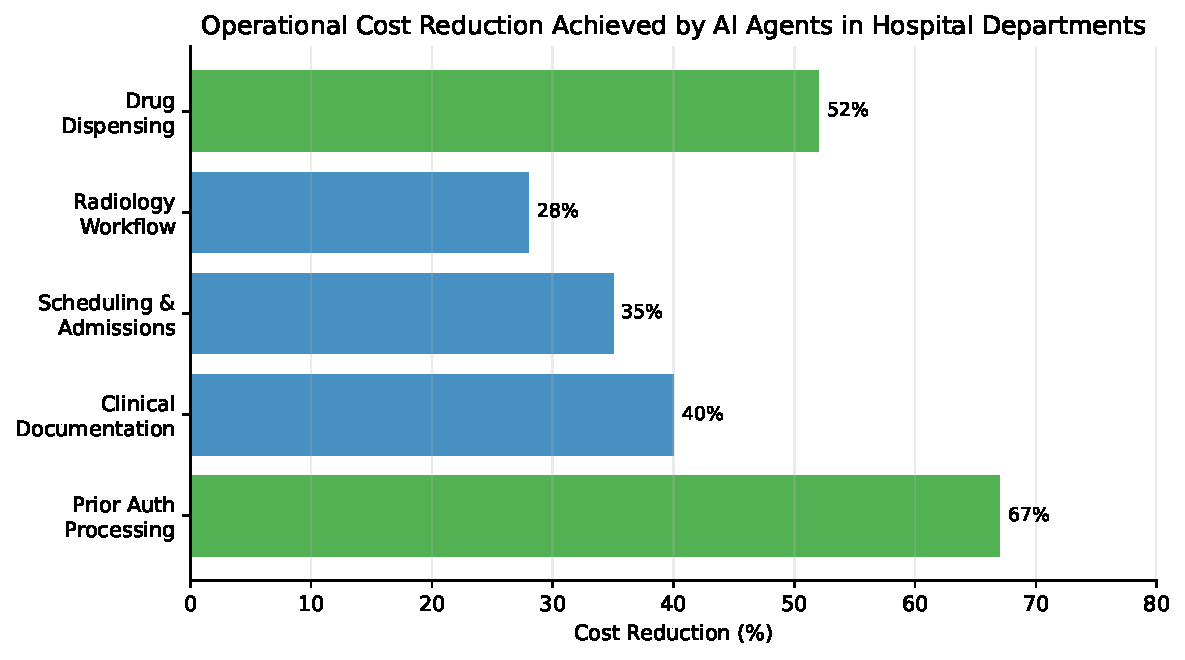
\includegraphics[width=0.88\textwidth]{../assets/graphs/cost_reduction.pdf}
  \caption{Operational cost reduction across hospital departments with the integration of AI agents. Significant reductions are observed in administrative tasks, supply chain management, and diagnostic processes \cite{dataart_digital_transformation}.}
  \label{fig:cost_reduction}
\end{figure}

\section{Future Outlook and Human-AI Collaboration}
\label{sec:future_outlook}
The future of AI agents in healthcare is characterized by continued innovation, with a strong emphasis on enhancing human-AI collaboration and developing more sophisticated, ethical systems. This section explores anticipated developments and the evolving paradigm of human-AI synergy.

\subsection{Advancements in Multi-Agent Systems}
\label{subsec:multi_agent_systems}
Future developments in AI agents will likely focus on multi-agent systems, where multiple AI agents collaborate to achieve complex healthcare goals. For example, one agent might specialize in diagnostic image analysis, another in genomic data interpretation, and a third in personalized treatment recommendations. These agents would interact and share insights, providing a more comprehensive and integrated approach to patient care \cite{russell2010artificial}. This collaborative model mirrors human multidisciplinary teams.

Such systems could also extend to coordinating care across different healthcare settings, from hospitals to home care. A multi-agent system could manage patient transitions, ensure continuity of care, and optimize resource allocation in real-time. The synergy between specialized AI agents promises to unlock new levels of efficiency and effectiveness in healthcare delivery, addressing systemic challenges through distributed intelligence.

\subsection{Explainable AI (XAI) and Trust}
\label{subsec:explainable_ai}
The "black box" nature of many deep learning models remains a barrier to widespread adoption in critical healthcare applications. Future advancements will prioritize Explainable AI (XAI), which aims to make AI decisions more transparent and understandable to human users \cite{goodfellow2016deep}. XAI techniques will allow clinicians to comprehend the reasoning behind an AI agent's recommendations, fostering greater trust and enabling more informed clinical judgment.

Increased transparency is crucial for ethical considerations, regulatory compliance, and building confidence among healthcare professionals and patients. When an AI agent can explain its diagnostic rationale or treatment suggestion, it empowers clinicians to validate the advice and integrate it more effectively into their practice. This shift from opaque predictions to interpretable insights is fundamental for the responsible deployment of AI in healthcare.

\subsection{Seamless Human-AI Collaboration}
\label{subsec:human_ai_collaboration}
The ultimate goal for AI agents in healthcare is to achieve seamless human-AI collaboration, where AI augments human capabilities rather than replacing them. This involves designing interfaces and workflows that facilitate intuitive interaction between clinicians and AI systems. AI agents will act as intelligent assistants, providing timely information, automating routine tasks, and offering expert insights to support human decision-making \cite{topol2019highperformance}. This partnership aims to leverage the strengths of both humans and AI.

For example, an AI agent might pre-analyze medical images, highlighting suspicious areas for a radiologist to review, thereby improving efficiency and reducing diagnostic errors. In surgical settings, robotic assistants can provide precision and stability, while human surgeons maintain overall control and strategic decision-making. This collaborative paradigm ensures that human empathy, critical thinking, and ethical judgment remain central to patient care, enhanced by AI's analytical power.

\section{Evaluating AI Agent Performance}
\label{sec:evaluating_performance}
The effectiveness of AI agents in healthcare must be rigorously evaluated to ensure their reliability and clinical utility. This involves using appropriate metrics that capture various aspects of performance, particularly in diagnostic applications. This section discusses key evaluation metrics and their importance.

\subsection{Metrics for Diagnostic Performance}
\label{subsec:diagnostic_metrics}
Evaluating the diagnostic performance of AI agents typically involves metrics such as accuracy, precision, recall, and F1-score. Accuracy measures the proportion of correct predictions (both true positives and true negatives) out of all predictions. However, accuracy alone can be misleading in cases of imbalanced datasets, where one class is much more prevalent than another. For instance, if a disease is rare, an AI could achieve high accuracy by simply predicting "no disease" for most cases.

Precision, also known as positive predictive value, measures the proportion of true positive predictions among all positive predictions made by the AI. Recall, or sensitivity, measures the proportion of true positive predictions among all actual positive cases. Both precision and recall are crucial for understanding an AI's ability to correctly identify disease while minimizing false positives and false negatives. A high recall is often prioritized in screening for serious conditions to avoid missing cases.

\subsection{The F1-Score Formula}
\label{subsec:f1_score_formula}
The F1-score is a harmonic mean of precision and recall, providing a single metric that balances both. It is particularly useful when there is an uneven class distribution, as it penalizes models that perform poorly on either precision or recall. A high F1-score indicates that the AI agent has both low false positives and low false negatives, making it a robust indicator of diagnostic performance.

The formula for the F1-score is defined as:
\begin{equation}
F1 = 2 \times \frac{\text{Precision} \times \text{Recall}}{\text{Precision} + \text{Recall}}
\label{eq:f1_score}
\end{equation}
Here, Precision is $\frac{\text{True Positives}}{\text{True Positives} + \text{False Positives}}$ and Recall is $\frac{\text{True Positives}}{\text{True Positives} + \text{False Negatives}}$. This formula ensures that a model must achieve a good balance between correctly identifying positive cases and avoiding incorrect positive identifications. The F1-score is widely used in medical AI research to provide a comprehensive assessment of model effectiveness.

\subsection{Validation and Continuous Monitoring}
\label{subsec:validation_monitoring}
Beyond initial evaluation, continuous validation and monitoring are essential for AI agents deployed in clinical settings. AI models can drift over time due to changes in patient populations, medical practices, or data input characteristics. Regular re-evaluation against new, independent datasets is necessary to ensure sustained performance \cite{fda_ai_ml_samd}. This ongoing process helps to detect any degradation in accuracy or emergence of new biases.

Post-market surveillance involves tracking the real-world performance of AI agents and collecting feedback from clinicians. This feedback loop is vital for identifying unforeseen issues, refining algorithms, and ensuring that the AI remains clinically relevant and safe. The Total Product Lifecycle approach advocated by regulatory bodies underscores the importance of this continuous monitoring for adaptive AI systems.

\section{Challenges and Limitations of AI Agents}
\label{sec:challenges_limitations}
Despite their transformative potential, AI agents in healthcare face significant challenges and limitations that must be acknowledged and addressed. These range from technical hurdles to broader societal and practical constraints.

\subsection{Data Quality and Availability}
\label{subsec:data_quality}
The performance of AI agents is heavily dependent on the quality, quantity, and representativeness of the data used for training. Healthcare data are often fragmented, incomplete, and inconsistent, making it difficult to build robust AI models \cite{davenport2019ai}. Issues such as missing values, incorrect entries, and varied data formats can introduce noise and bias into the training process. Poor data quality directly translates to unreliable AI predictions.

Furthermore, access to large, diverse, and ethically sourced medical datasets is a persistent challenge. Data sharing is often restricted by privacy regulations and proprietary concerns, limiting the scope and generalizability of AI models. Overcoming these data-related limitations requires significant investment in data standardization, curation, and secure sharing platforms.

\subsection{Integration Complexity and Interoperability}
\label{subsec:integration_complexity}
Integrating AI agents into existing, often legacy, healthcare IT systems is a complex endeavor. Healthcare environments are characterized by a patchwork of different software systems, electronic health records (EHRs), and medical devices that often lack seamless interoperability \cite{dataart_digital_transformation}. This fragmentation makes it difficult for AI agents to access and synthesize information from all relevant sources, hindering their ability to provide comprehensive insights.

Achieving true interoperability requires standardized APIs, common data models, and robust integration platforms. The technical and organizational challenges associated with this integration can be substantial, requiring significant resources and strategic planning. Without effective integration, AI agents may operate in silos, limiting their impact and creating additional workflow complexities for clinicians.

\subsection{Ethical and Societal Acceptance}
\label{subsec:ethical_societal_acceptance}
Beyond technical and regulatory hurdles, the ethical and societal acceptance of AI agents in healthcare remains a critical limitation. Concerns about data privacy, algorithmic bias, and accountability for errors can erode public trust \cite{nih_ethical_implications}. Patients and clinicians may be hesitant to adopt AI solutions if they do not understand how these systems work or if they perceive a lack of human oversight.

The potential for dehumanization of care, where technology might diminish the empathetic human connection between patients and providers, is another significant concern \cite{who2021ai}. Addressing these ethical and societal anxieties requires transparent communication, public education, and the active involvement of diverse stakeholders in the development and deployment of AI. Building trust is paramount for the widespread and beneficial adoption of AI in healthcare.

\section{AI Agent System Architecture for Personalized Treatment}
\label{sec:ai_architecture}
The design of AI agent systems for personalized treatment planning involves a sophisticated architecture that integrates various data sources and AI modules. This architecture ensures comprehensive analysis and tailored recommendations.

\subsection{Data Ingestion and Preprocessing}
\label{subsec:data_ingestion}
The initial stage of an AI agent system for personalized treatment involves ingesting diverse patient data. This includes Electronic Health Records (EHRs), which contain medical history, diagnoses, medications, and lab results \cite{zynxhealth_clinical_decision_support}. Genomic data, providing insights into an individual's genetic predispositions and drug metabolism, are also crucial inputs. Additionally, lifestyle data from wearable devices or patient-reported outcomes can offer valuable context.

Once ingested, the raw data undergo extensive preprocessing. This involves cleaning, normalization, and feature extraction to transform heterogeneous data into a standardized format suitable for AI model input. Data quality checks are performed to identify and handle missing values or inconsistencies. This meticulous preprocessing step is vital for ensuring the accuracy and reliability of subsequent AI analyses.

\subsection{AI Processing Modules}
\label{subsec:ai_processing}
The core of the system consists of multiple AI processing modules, each specialized for different analytical tasks. Machine learning models, particularly deep learning networks, are used for pattern recognition in complex data. For instance, a module might analyze genomic sequences to identify disease markers or predict drug efficacy based on genetic variations \cite{wang2019deep}. Another module could process time-series data from EHRs to predict disease progression.

Natural Language Processing (NLP) modules extract relevant information from unstructured clinical notes and medical literature. This allows the system to synthesize qualitative data and incorporate the latest research findings into its recommendations \cite{shah2019artificial}. Reinforcement learning agents might be employed to simulate various treatment pathways and learn optimal strategies for individual patients, considering their unique profiles and responses.

\subsection{Output and Recommendation Generation}
\label{subsec:output_recommendation}
The final stage involves generating actionable outputs and personalized treatment recommendations. This includes tailored drug dosages, specific therapeutic interventions, and preventive strategies based on the patient's risk profile. The system also provides risk assessments, highlighting potential adverse drug reactions or disease complications. These outputs are presented in a clear, interpretable format for clinicians.

Crucially, the system incorporates Explainable AI (XAI) components to provide a rationale for its recommendations. This transparency allows healthcare providers to understand the underlying evidence and logic, facilitating informed decision-making and fostering trust in the AI agent's advice. The goal is to augment the clinician's expertise with data-driven insights, leading to optimized patient outcomes.

\begin{figure}[H]
  \centering
  \begin{tikzpicture}[node distance=2cm, auto, >=Stealth, thick]
    % Nodes
    \node (start) [rectangle, rounded corners, draw, fill=blue!10, text width=2.5cm, minimum height=1cm, text centered] {Data Ingestion};
    \node (ehr) [rectangle, draw, fill=gray!10, below=0.7cm of start, xshift=-1.5cm, text width=2.5cm, minimum height=0.8cm, text centered] {EHR Data};
    \node (genomics) [rectangle, draw, fill=gray!10, below=0.7cm of start, xshift=1.5cm, text width=2.5cm, minimum height=0.8cm, text centered] {Genomic Data};
    \node (preprocessing) [rectangle, rounded corners, draw, fill=blue!10, below=1.5cm of start, text width=2.5cm, minimum height=1cm, text centered] {Data Preprocessing};
    \node (ml_models) [rectangle, draw, fill=green!10, right=2cm of preprocessing, text width=2.5cm, minimum height=1cm, text centered] {ML Models};
    \node (nlp_module) [rectangle, draw, fill=green!10, above=0.7cm of ml_models, text width=2.5cm, minimum height=1cm, text centered] {NLP Module};
    \node (rl_agent) [rectangle, draw, fill=green!10, below=0.7cm of ml_models, text width=2.5cm, minimum height=1cm, text centered] {RL Agent};
    \node (ai_processing) [rectangle, rounded corners, draw, fill=blue!20, right=2cm of preprocessing, text width=3.5cm, minimum height=3cm, text centered, label={[font=\small]above:AI Processing Modules}] {};
    \node (output) [rectangle, rounded corners, draw, fill=blue!10, right=2cm of ai_processing, text width=2.5cm, minimum height=1cm, text centered] {Output Generation};
    \node (treatment_rec) [rectangle, draw, fill=gray!10, below=0.7cm of output, xshift=-1.5cm, text width=2.5cm, minimum height=0.8cm, text centered] {Treatment Recommendations};
    \node (risk_assessment) [rectangle, draw, fill=gray!10, below=0.0cm of output, xshift=1.5cm, text width=2.5cm, minimum height=0.8cm, text centered] {Risk Assessment};
    \node (xai) [rectangle, draw, fill=orange!10, above=0.7cm of output, text width=2.5cm, minimum height=0.8cm, text centered] {Explainable AI (XAI)};

    % Positioning ML, NLP, RL inside AI Processing
    \coordinate (ml_center) at (ml_models.center);
    \coordinate (nlp_center) at (nlp_module.center);
    \coordinate (rl_center) at (rl_agent.center);
    \node at (ml_center) {ML Models};
    \node at (nlp_center) {NLP Module};
    \node at (rl_center) {RL Agent};

    % Arrows
    \draw[->] (ehr) -- (preprocessing) node[midway, above, fill=white, inner sep=2pt, font=\footnotesize] {Patient Data};
    \draw[->] (genomics) -- (preprocessing);
    \draw[->] (preprocessing) -- (ai_processing) node[midway, above, fill=white, inner sep=2pt, font=\footnotesize] {Cleaned Data};
    \draw[->] (ai_processing) -- (output) node[midway, above, fill=white, inner sep=2pt, font=\footnotesize] {Processed Insights};
    \draw[->] (output) -- (treatment_rec) node[midway, right, fill=white, inner sep=2pt, font=\footnotesize] {Personalized Plans};
    \draw[->] (output) -- (risk_assessment) node[midway, right, fill=white, inner sep=2pt, font=\footnotesize] {Risk Profiles};
    \draw[->] (ai_processing) -- (xai) node[midway, above, fill=white, inner sep=2pt, font=\footnotesize] {Interpretability Data};
    \draw[->] (xai) -- (output) node[midway, above, fill=white, inner sep=2pt, font=\footnotesize] {Explanations};
  \end{tikzpicture}
  \caption{Architectural diagram of an AI agent system for personalized treatment planning. The system integrates diverse data sources, processes them through specialized AI modules, and generates actionable, explainable recommendations \cite{topol2019deep}.}
  \label{fig:ai_architecture}
\end{figure}

\section{\texthebrew{סוכני בינה מלאכותית בשירותי הבריאות: היבטים דו-לשוניים}}
\label{sec:bidi_ai_healthcare}
\begin{hebrewblock}
סעיף זה מציג את ההיבטים הדו-לשוניים של סוכני בינה מלאכותית בשירותי הבריאות, תוך התמקדות בשימוש בשפה העברית. השילוב של בינה מלאכותית בסביבות רפואיות בישראל דורש התייחסות מיוחדת לשפה ולתרבות המקומית. הבנה מעמיקה של טקסטים רפואיים בעברית חיונית לפיתוח סוכנים יעילים.
\end{hebrewblock}
\begin{englishblock}
This section presents the bilingual aspects of AI agents in healthcare, focusing on the use of the Hebrew language. The integration of AI in medical environments in Israel requires special attention to the local language and culture. A deep understanding of medical texts in Hebrew is essential for developing effective agents.
\end{englishblock}

\subsection{\texthebrew{אתגרי עיבוד שפה טבעית בעברית}}
\label{subsec:hebrew_nlp_challenges}
\begin{hebrewblock}
עיבוד שפה טבעית (NLP) בעברית מציב אתגרים ייחודיים עבור סוכני בינה מלאכותית. השפה העברית היא שפה שמית בעלת מורפולוגיה עשירה, כתיב חסר ודו-כיווניות (מימין לשמאל). מאפיינים אלו מקשים על מודלים סטנדרטיים של NLP שפותחו בעיקר עבור שפות לטיניות. פיתוח מודלים ייעודיים לעברית הוא הכרחי.
\end{hebrewblock}
\begin{englishblock}
Natural Language Processing (NLP) in Hebrew presents unique challenges for AI agents. Hebrew is a Semitic language with rich morphology, unvocalized script, and right-to-left directionality. These characteristics complicate standard NLP models primarily developed for Latin-based languages. Developing specialized models for Hebrew is essential.
\end{englishblock}

\subsection{\texthebrew{הטמעת סוכני בינה מלאכותית בבתי חולים בישראל}}
\label{subsec:ai_implementation_israel}
\begin{hebrewblock}
הטמעת סוכני בינה מלאכותית בבתי חולים בישראל דורשת התאמה למערכות המידע הקיימות ולתרבות העבודה המקומית. מערכות רפואיות רבות בישראל משתמשות בעברית, ולכן סוכני בינה מלאכותית חייבים להיות מסוגלים לעבד ולהפיק מידע בשפה זו. הכשרת צוותים רפואיים לשימוש בסוכנים אלו בעברית היא קריטית.
\end{hebrewblock}
\begin{englishblock}
Implementing AI agents in Israeli hospitals requires adaptation to existing information systems and local work culture. Many medical systems in Israel use Hebrew, so AI agents must be able to process and generate information in this language. Training medical teams to use these agents in Hebrew is crucial.
</englishblock>

\subsection{\texthebrew{היבטים אתיים ותרבותיים מקומיים}}
\label{subsec:local_ethical_cultural}
\begin{hebrewblock}
היבטים אתיים ותרבותיים מקומיים משפיעים על פיתוח ופריסת סוכני בינה מלאכותית בישראל. יש להתחשב בנורמות תרבותיות, רגישויות דתיות וחברתיות בעת עיצוב מערכות AI. הבטחת פרטיות נתונים ואלגוריתמים הוגנים, תוך התאמה לחוקים ולתקנות הישראליים, היא בעלת חשיבות עליונה.
\end{hebrewblock}
\begin{englishblock}
Local ethical and cultural aspects influence the development and deployment of AI agents in Israel. Cultural norms, religious sensitivities, and social considerations must be taken into account when designing AI systems. Ensuring data privacy and fair algorithms, while adhering to Israeli laws and regulations, is of paramount importance.
</englishblock}

\section{Conclusion}
\label{sec:conclusion}
AI agents are poised to fundamentally reshape healthcare, offering unprecedented opportunities to enhance diagnostic accuracy, personalize treatments, and optimize operational efficiencies. This article has explored their diverse applications, from image analysis to administrative automation, highlighting the sophisticated machine learning, natural language processing, and sensor fusion technologies that underpin their capabilities. The transformative potential of these agents is evident in their ability to augment human expertise and streamline complex medical processes.

However, the successful and ethical integration of AI agents hinges on a proactive approach to addressing inherent challenges. Critical ethical considerations, including data privacy, algorithmic bias, and accountability for errors, demand robust frameworks and continuous vigilance. Furthermore, the evolving global regulatory landscape underscores the need for clear guidelines and continuous oversight to ensure patient safety and trust. Finally, the practical implementation requires substantial investment in infrastructure, comprehensive workforce retraining, and effective change management strategies. By navigating these complexities thoughtfully, healthcare systems can harness the full power of AI agents to deliver higher quality, more equitable, and more efficient patient care.

\printbibliography[heading=bibintoc]

\end{document}